\begin{problem}{/images/problems/pic.jpg}{Table of Numbers}We have a $5 \times 7$ table and we wish to put $1$ or $-1$ in each of its cells, so that the product of the numbers of each row becomes $-1$ and the product of the numbers of each column becomes $-1$ (similar to the figure below). How many different ways can we do that?\\[0.2cm]

\textbf{Additional problem}: What if the table is $15 \times 16$?

\begin{center}
	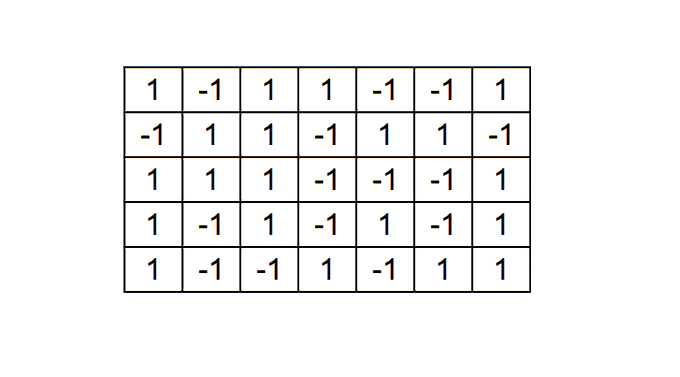
\includegraphics[width=9cm]{/images/problems/39_grid.png}
\end{center}

Link to the problem on Twitter:  \url{https://twitter.com/Riazi_Cafe/status/1704369917871690162}\end{problem}
\begin{solution}
The correct answer is $2^{24}$ for the $5 \times 7$ table and 0 for the $15 \times 16$ table.

Notice that in the figure below, if the values written on the blue part are known, we can determine the values of the yellow part and the red part uniquely so that the product of the values of each column is equal to -1 and the product of the values of each row is equal to -1.

\begin{center}
	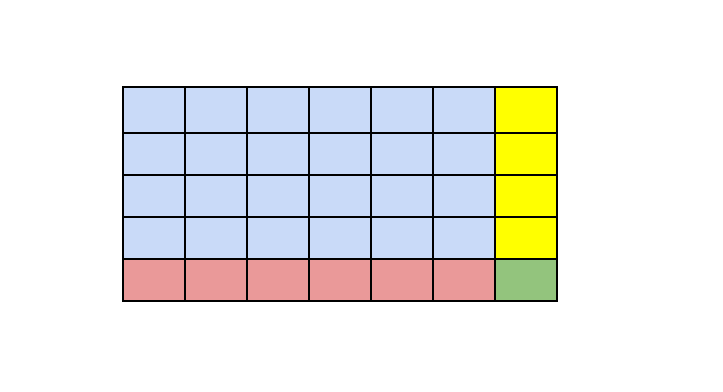
\includegraphics[width=9cm]{/images/problems/39_diagram0.png}
\end{center}


For example, to determine the value of the yellow cell in the first row, we can multiply the values of the first row, and then multiply the result by -1 and place it there.
We can also determine the value of the green cell uniquely by using the yellow or red part so that the product of the last column and the product of the last row becomes -1. Thus by determining the blue part, the rest of the table to will have a unique assignment that satisfies our criteria. The blue section has 24 cells and we have 2 choices for each cell, so we have $2^{24}$ ways.\\[0.2cm]



In the case of  $15 \times 16$ table, the answer is zero, since the parity of the number of rows and columns is not the same. More precisely, if the multiplication of the values in each row is $-1$, then since we have 15 rows, the multiplication of the values of the table would be equal to $(-1)^{15} = -1$. Similarly, if the multiplication of the values in each column is $-1$, since we have 16 columns, then the multiplication of all values of the table should be equal to $(-1)^{16} = 1$. Thus, both conditions cannot be satisfied simultaneously.


\end{solution}
